\documentclass[aspectratio=169]{beamer}

\usepackage[T1]{fontenc}
\usepackage[utf8]{inputenc}
\usepackage[english]{babel}
\usepackage{pgfplots}
\pgfplotsset{compat=newest}
\usepackage{booktabs}
\usepackage{siunitx}
\usepackage{subcaption}
\usepackage{multirow}
\usepackage{lmodern}
\usepackage{charter} % serif

\usetheme[department=compute]{DTU}

\title[02456 Deep Learning]{Deep Convolutional and Recurrent Neural Networks for Interpretable Analysis of EEG Sleep Stage Scoring}
\author{Anders Launer Baek}
\institute{DTU Compute, Technical University of Denmark}
\date{\today}
	
\newcommand{\tabitem}{{\color{dtured}$\bullet$} }

\begin{document}
\frame{
	\maketitle
}

%\frame{
%	\frametitle{Outline}
%	\tableofcontents
%}


\section{The Challenge}
\subsection{Sleeping Stages}
\frame{
	\frametitle{Sleeping Stages}
	\begin{figure}[th!]
\centering
\begin{subfigure}{.16\textwidth}
  \centering
  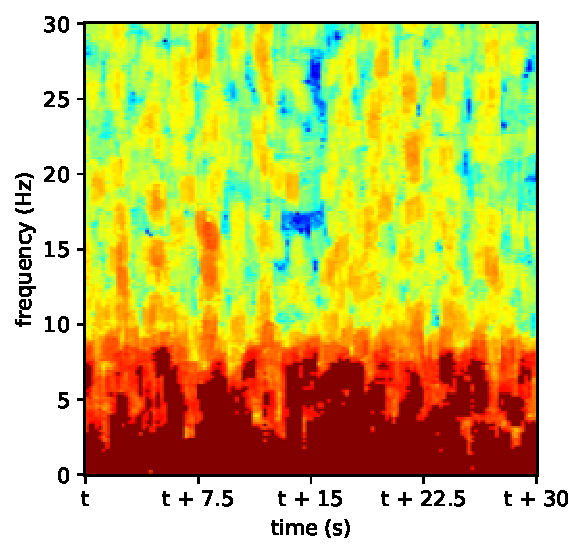
\includegraphics[width=1\linewidth]{./../Article/pics/class_clean_0}
  \caption{W}
  \label{fig_1_11}
\end{subfigure}%
\begin{subfigure}{.16\textwidth}
  \centering
  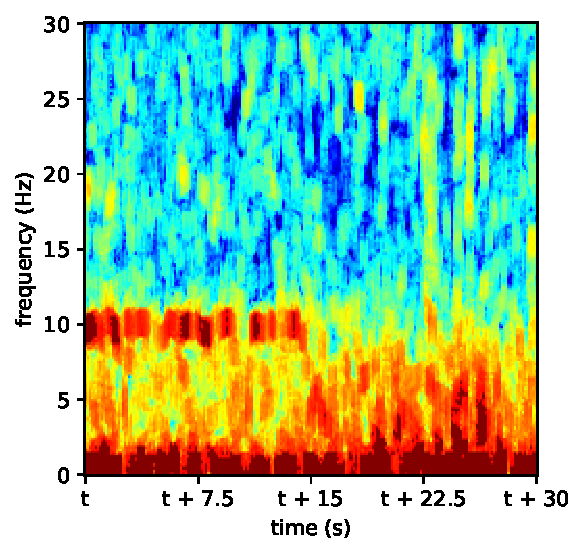
\includegraphics[width=1\linewidth]{./../Article/pics/class_clean_1}
  \caption{N1}
  \label{fig_1_12}
\end{subfigure}%
\begin{subfigure}{.16\textwidth}
  \centering
  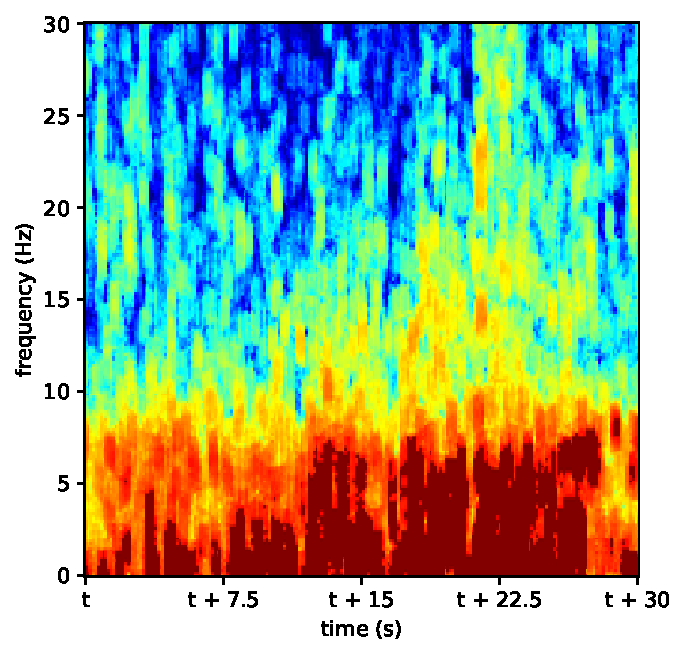
\includegraphics[width=1\linewidth]{./../Article/pics/class_clean_2}
  \caption{N2}
  \label{fig_1_13}
\end{subfigure}%
\begin{subfigure}{.16\textwidth}
  \centering
  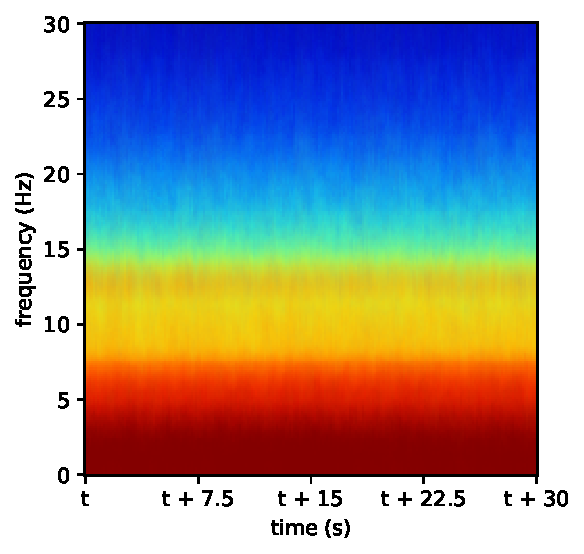
\includegraphics[width=1\linewidth]{./../Article/pics/class_clean_3}
  \caption{N3}
  \label{fig_1_14}
\end{subfigure}%
\begin{subfigure}{.16\textwidth}
  \centering
  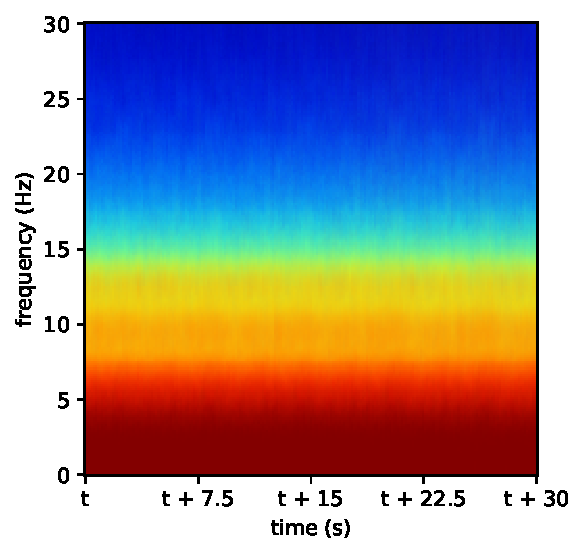
\includegraphics[width=1\linewidth]{./../Article/pics/class_clean_4}
  \caption{N4}
  \label{fig_1_15}
\end{subfigure}%
\begin{subfigure}{.16\textwidth}
  \centering
  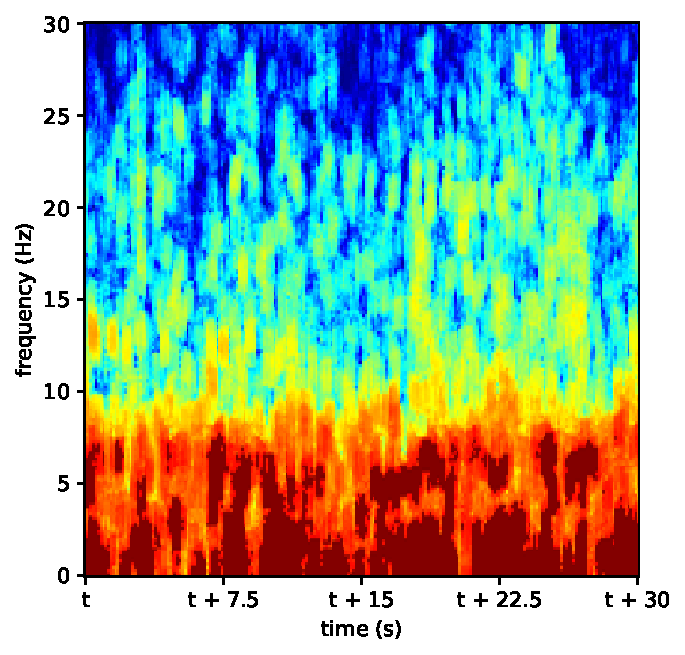
\includegraphics[width=1\linewidth]{./../Article/pics/class_clean_5}
  \caption{R}
  \label{fig_1_16}
\end{subfigure}

\caption{This figure illustrates a random epoch of the multi-taper spectrum for each sleeping stage. There is high similarity between sleeping stage N3 and N4.}
\label{fig_1}
\end{figure}


\begin{table}[th!]
\begin{tabular}{l|llllll}
Sleep Stage & W & N1 &  N2& N3 & N4 & R \\\hline
Dist. (in \%) &12 &7&46&9&6&20
\end{tabular}
\caption{This table summerises the aggregates the distribution of the labels for all 20 Subjects. The distribution of the labels illustrates the sleep stages of subjects during the recordings.}
\label{tab_class_balance}
\end{table}


}





\section{Performance}

\frame{
	\frametitle{Confusion Matrices}
\begin{table}[th!]
\centering
\begin{tabular}{ll | llllll | llllll }
                     &    & \multicolumn{6}{c}{Predicted} & \multicolumn{6}{| c}{Normalized pred. (in \%)} \\
                     &    & W  & N1  & N2  & N3  & N4 & R & W & N1 & N2 & N3 & N4 & R \\\hline
\multirow{6}{*}{CNN} & W  &495 & 145 & 29 & 11 & 1 & 20 & 71 & 21 & 4 & 2 & 0 & 3  \\ 
                     & N1 &    25 & 211 & 43 & 0 & 0 & 62 & 7 & 62 & 13 & 0 & 0 & 18  \\ 
                     & N2 &    4 & 51 & 1313 & 104 & 17 & 68 & 0 & 3 & 84 & 7 & 1 & 4 \\ 
                     & N3 &    0 & 2 & 11 & 164 & 64 & 0 & 0 & 1 & 5 & 68 & 27 & 0  \\ 
                     & N4 &    0 & 0 & 0 & 54 & 91 & 0 & 0 & 0 & 0 & 37 & 63 & 0  \\ 
                     & R  &    17 & 80 & 46 & 0 & 0 & 591 & 2 & 11 & 6 & 0 & 0 & 81 \\ \hline
\multirow{6}{*}{RNN} & W  &    578 & 39 & 26 & 7 & 1 & 43 & 83 & 6 & 4 & 1 & 0 & 6 \\ 
                     & N1 &    38 & 107 & 64 & 0 & 0 & 132 & 11 & 31 & 19 & 0 & 0 & 39 \\ 
                     & N2 &    8 & 13 & 1314 & 102 & 28 & 92 & 1 & 1 & 84 & 7 & 2 & 6 \\ 
                     & N3 &    3 & 0 & 18 & 125 & 95 & 0 & 1 & 0 & 7 & 52 & 39 & 0  \\ 
                     & N4 &    0 & 0 & 1 & 60 & 84 & 0 & 0 & 0 & 1 & 41 & 58 & 0  \\ 
                     & R  &    19 & 36 & 43 & 0 & 0 & 636 & 3 & 5 & 6 & 0 & 0 & 87
\end{tabular}
\caption{Confusion matrix and normalized confusion matrix for the CNN and RNN network.}
\label{tab_res_1}
\end{table}
	
	
}


\frame{
	\frametitle{Bootstrapped Performances Metrics}
	\begin{table}[th!]
\centering
\begin{tabular}{l | llll}
Study & Precision & Sensitivity & F$_1$-score & Accuracy \\\hline
%\cite{main_ar}               & 65.4-\textbf{67.9}-70.4 & 70.9-\textbf{71.3}-71.8 & 67.5-\textbf{68.8}-70.0 & 92.3-\textbf{92.3}-92.4\\
CNN               & 65-\textbf{68}-70 & 71-\textbf{71}-72 & 67-\textbf{69}-70 & 92-\textbf{92}-92\\
RNN               & 62-\textbf{65}-67 & 63-\textbf{66}-69 & 62-\textbf{64}-67 & 92-\textbf{92}-92
\end{tabular}
\caption{\textbf{Mean} and corresponding $95\%$ confident values computed by 100.000 bootstrap iterations with replacement.}
\label{tab_res_2}
\end{table}
}

\frame{
	\frametitle{Sensitivity Maps}
	\begin{figure}[th!]
\centering
\begin{subfigure}{.16\textwidth}
  \centering
  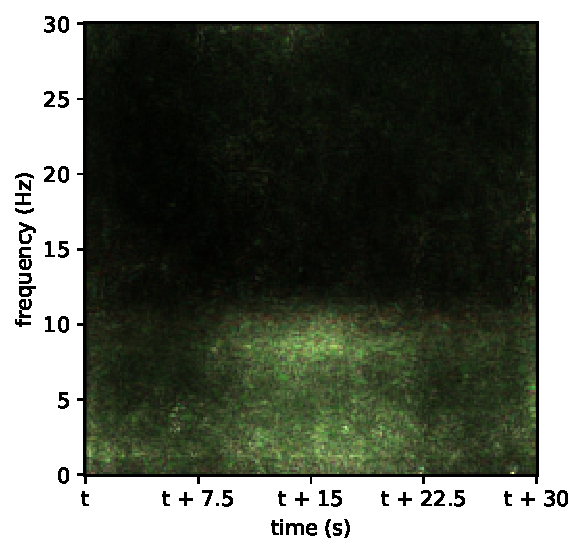
\includegraphics[width=1\linewidth]{./../Article/pics/class_master_0}
  \caption{W}
  \label{fig_1_21}
\end{subfigure}%
\begin{subfigure}{.16\textwidth}
  \centering
  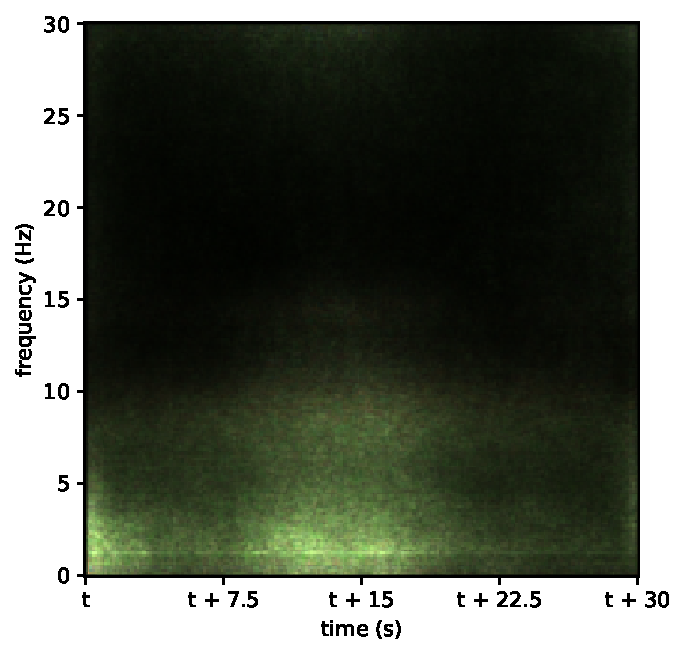
\includegraphics[width=1\linewidth]{./../Article/pics/class_master_1}
  \caption{N1}
  \label{fig_1_22}
\end{subfigure}%
\begin{subfigure}{.16\textwidth}
  \centering
  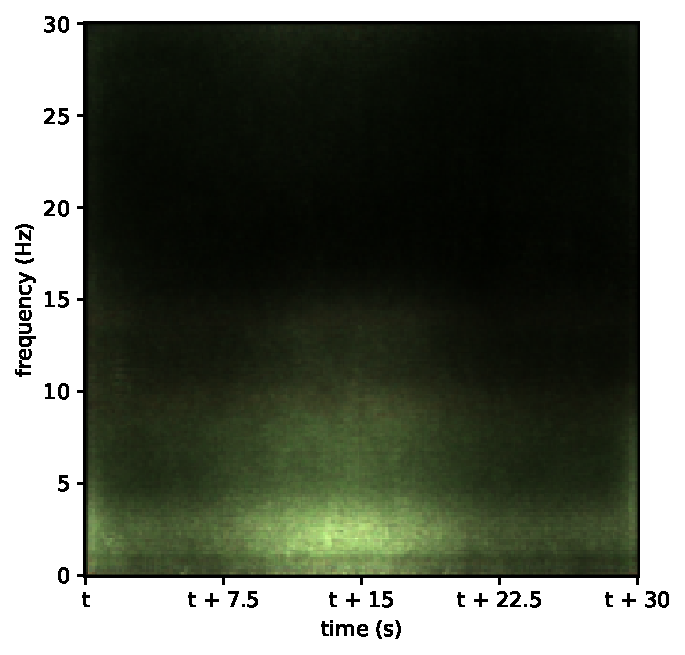
\includegraphics[width=1\linewidth]{./../Article/pics/class_master_2}
  \caption{N2}
  \label{fig_1_23}
\end{subfigure}%
\begin{subfigure}{.16\textwidth}
  \centering
  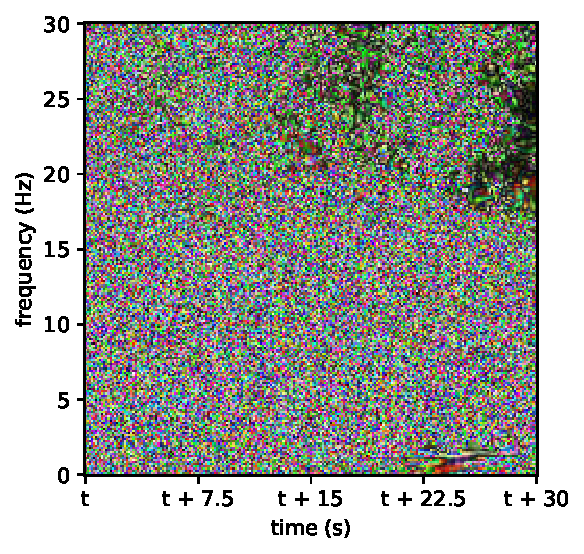
\includegraphics[width=1\linewidth]{./../Article/pics/class_master_3}
  \caption{N3}
  \label{fig_1_24}
\end{subfigure}%
\begin{subfigure}{.16\textwidth}
  \centering
  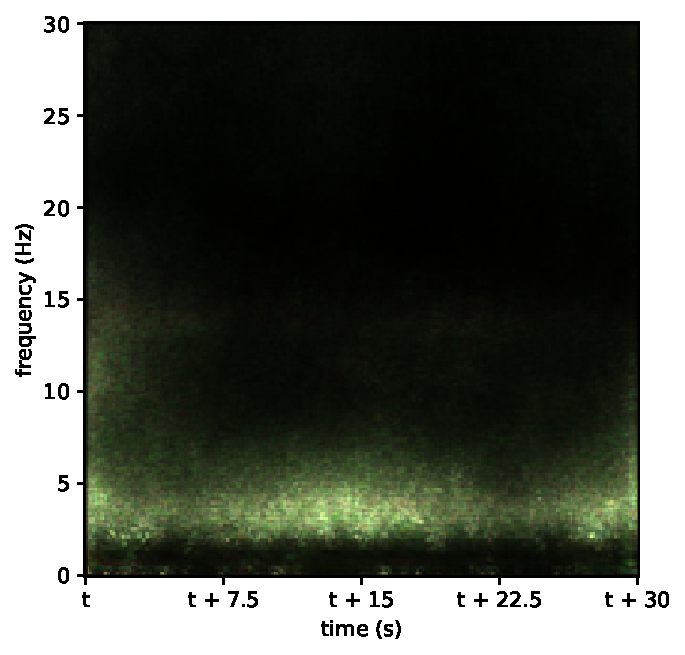
\includegraphics[width=1\linewidth]{./../Article/pics/class_master_4}
  \caption{N4}
  \label{fig_1_25}
\end{subfigure}%
\begin{subfigure}{.16\textwidth}
  \centering
  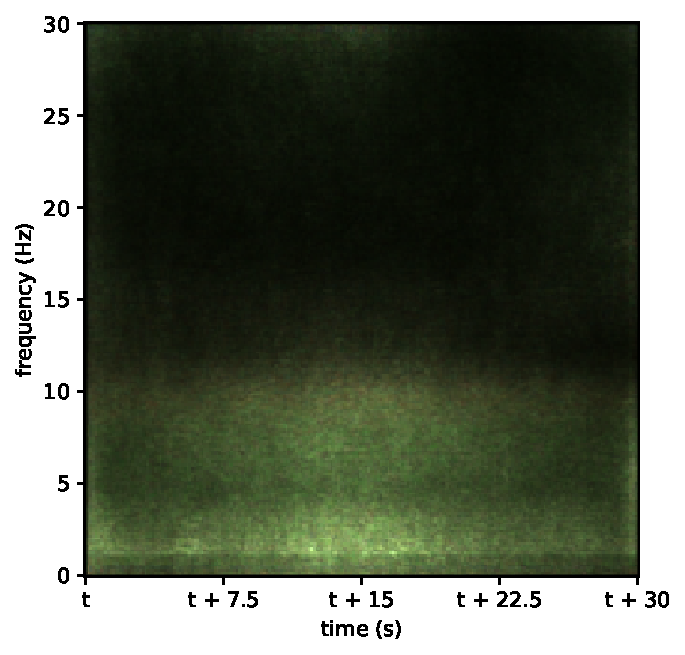
\includegraphics[width=1\linewidth]{./../Article/pics/class_master_5}
  \caption{R}
  \label{fig_1_26}
\end{subfigure}


\begin{subfigure}{.16\textwidth}
  \centering
  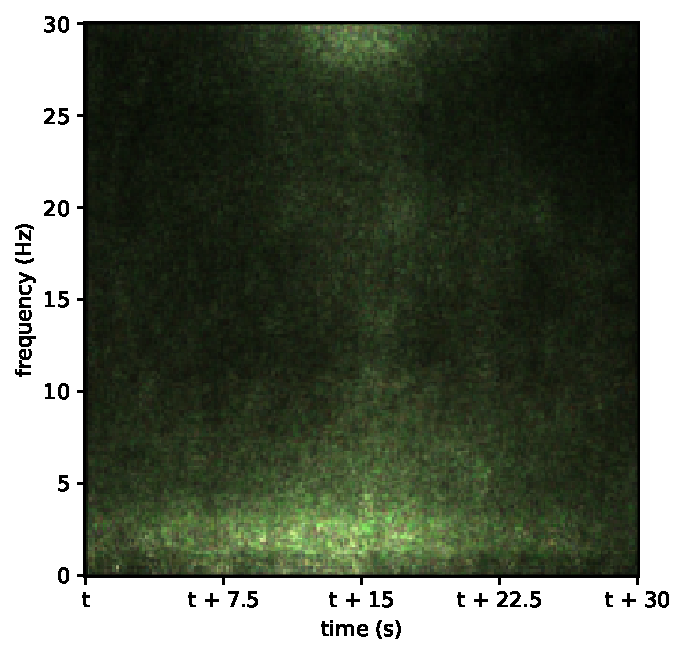
\includegraphics[width=1\linewidth]{./../Article/pics/class_rnn_0}
  \caption{W}
  \label{fig_1_31}
\end{subfigure}%
\begin{subfigure}{.16\textwidth}
  \centering
  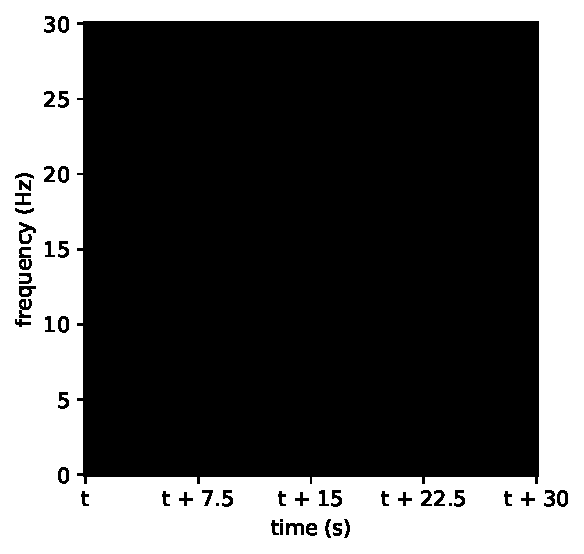
\includegraphics[width=1\linewidth]{./../Article/pics/class_rnn_1}
  \caption{N1}
  \label{fig_1_32}
\end{subfigure}%
\begin{subfigure}{.16\textwidth}
  \centering
  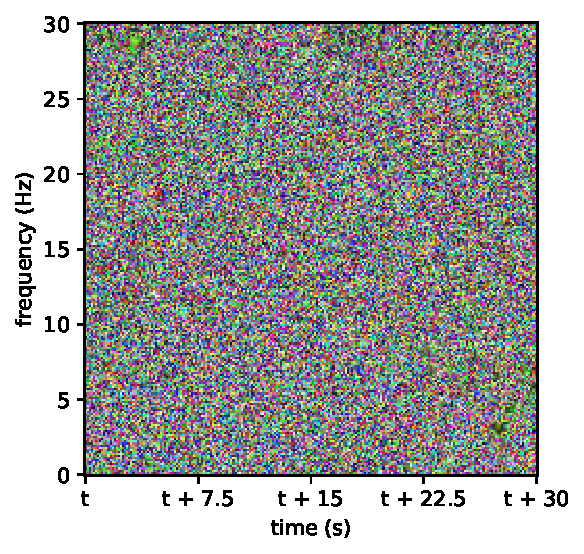
\includegraphics[width=1\linewidth]{./../Article/pics/class_rnn_2}
  \caption{N2}
  \label{fig_1_33}
\end{subfigure}%
\begin{subfigure}{.16\textwidth}
  \centering
  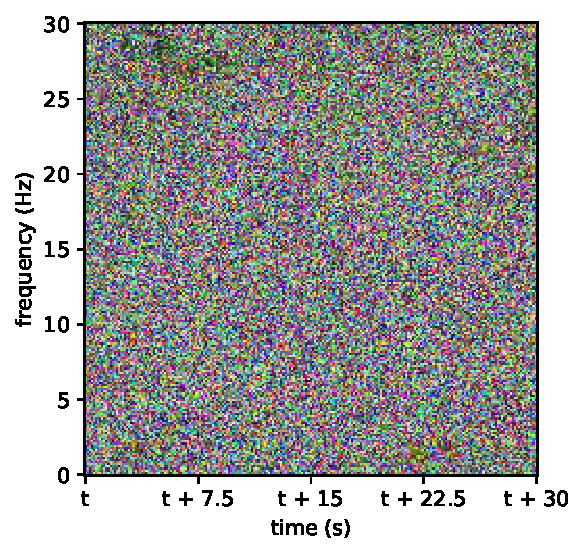
\includegraphics[width=1\linewidth]{./../Article/pics/class_rnn_3}
  \caption{N3}
  \label{fig_1_34}
\end{subfigure}%
\begin{subfigure}{.16\textwidth}
  \centering
  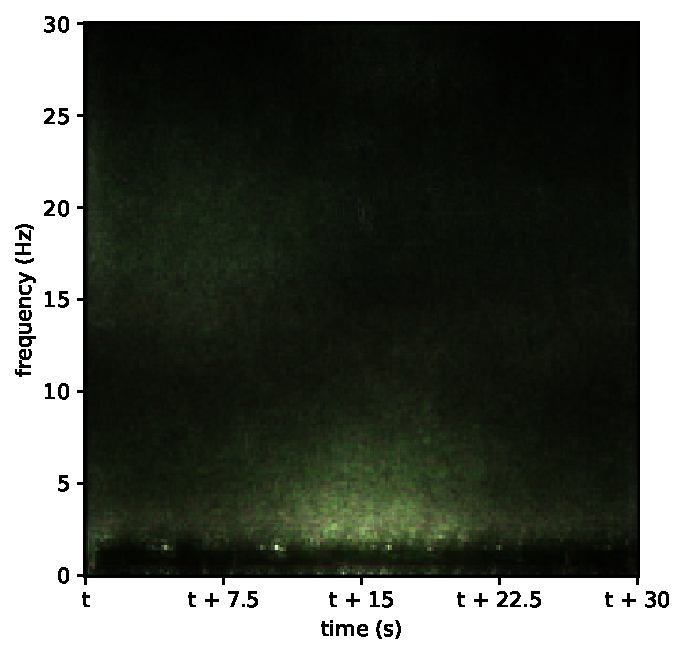
\includegraphics[width=1\linewidth]{./../Article/pics/class_rnn_4}
  \caption{N4}
  \label{fig_1_35}
\end{subfigure}%
\begin{subfigure}{.16\textwidth}
  \centering
  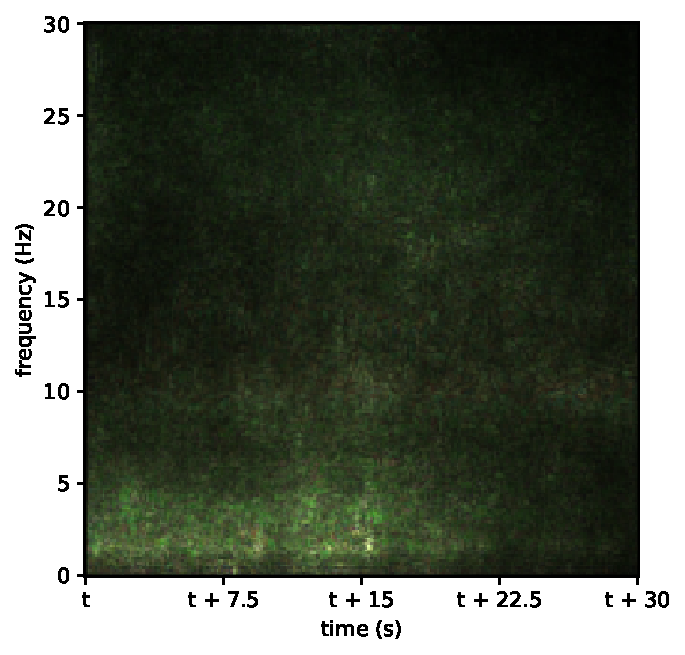
\includegraphics[width=1\linewidth]{./../Article/pics/class_rnn_5}
  \caption{R}
  \label{fig_1_36}
\end{subfigure}

\caption{This figure illustrates a random epoch of the multi-taper spectrum for each sleeping stage. There is high similarity between sleeping stage N3 and N4.}
\label{fig_2}
\end{figure}
}




% ads
\section{Conclusion}
\subsection{Conclusion}
\frame{
	\frametitle{Conclusion}
	
	\setbeamercovered{transparent}
	\begin{itemize}
		\item<1-> Watch the frame number.
		\item<2-> It doesn't change!
	\end{itemize}

	
}

\subsection{Future Research}
\frame{
	\frametitle{Future Research}
	\setbeamercovered{transparent}
	\begin{itemize}
		\item<1-> Watch the frame number.
		\item<2-> It doesn't change!
	\end{itemize}

}







%\section{Demonstration}
%\subsection{Lists}
%\frame{
%	\frametitle{Lists}
%	\begin{itemize}
%		\item Notice
%		\item the
%		\item red
%		\item bullet
%	\end{itemize}
%	
%	\begin{enumerate}
%		\item Wow
%		\item numbered
%		\item list
%	\end{enumerate}
%}
%
%\subsection{Blocks}
%\frame{
%	\frametitle{Blocks}
%	\begin{block}{Cool block}
%		Get nice visual effects by organizing content into \textbf{blocks}. Title background color matches the red from DTU logo.
%	\end{block}
%}
%
%\subsection{Tables}
%\frame{
%	\frametitle{Tables}
%	\begin{table}
%		\small
%		\caption{Not a regular table. Content is aligned with respect to the decimal symbol.}
%		\label{tab:S:standard}
%		\centering
%		\begin{tabular}{S}
%			\toprule
%			{Some Values} \\
%			\midrule
%			2.3456 \\
%			34.2345 \\
%			-6.7835 \\
%			90.473 \\
%			5642.5 \\
%			1.2e3 \\
%			e4 \\
%			\bottomrule
%		\end{tabular}
%	\end{table}
%}
%
%\subsection{Plots}
%\frame{
%	\frametitle{Plots}
%	Stunt your colleagues with amazing plots (pgfplots).
%	\begin{figure}[htbp]
%	\centering
%	\small
%	\begin{tikzpicture}
%		\begin{axis}[
%			width=0.4\textwidth,
%			grid=major,
%			title={Model Validation},
%			xlabel={X},
%			ylabel={Y}
%		]
%		
%		\addplot {-x^5 - 242};
%		\addlegendentry{model}
%	
%		\addplot coordinates {
%			(-4.77778,2027.60977)
%			(-3.55556,347.84069)
%			(-2.33333,22.58953)
%			(-1.11111,-493.50066)
%			(0.11111,46.66082)
%			(1.33333,-205.56286)
%			(2.55556,-341.40638)
%			(3.77778,-1169.24780)
%			(5.00000,-3269.56775)
%		};
%		\addlegendentry{estimate}
%		\end{axis}
%	\end{tikzpicture}
%	\end{figure}
%}

%\subsection{Frame Numbers}
%\frame{
%	\frametitle{Frame number instead of page number}
%	\setbeamercovered{transparent}
%	\begin{itemize}
%		\item<1-> Watch the frame number.
%		\item<2-> It doesn't change!
%	\end{itemize}
%}

{
%\setbeamercolor{background canvas}{bg=black} % Background color
%	\frame[dtuwhitelogo]{
%		\frametitle{Hello Blackness}
%		Here is another frame style!
%	}
%}


%================================================
%===  Define the contact details
\newcommand\contactTable{ %
  \begin{tabular}{lr}
    \multicolumn{2}{l}{Anders Launer Baek} \\ 
    s160159@student.dtu.dk \\
    \multicolumn{2}{l}{DTU Compute, Technical University of Denmark}
    %\multicolumn{2}{l}{DTU Compute, Technical University of Denmark} \\ \midrule
    %Building 308, Room 119    & latex-support@student.dtu.dk. \\
    %2800 Kgs. Lyngby, Denmark & +45 4525 phone \\
    %http://www.latex.dtu.dk   & +45 4525 fax
  \end{tabular}
}%

%\frame[dtuwhitelogo, bgfilename=dtu_bg_fiber]{
%  \begin{tikzpicture}[remember picture,overlay]
%    \node[fill=black, fill opacity=0.9, 
%          text=white, text opacity=1.0,
%          rounded corners=5pt, 
%          font=\scriptsize] at (current page.center) {\contactTable};
%  \end{tikzpicture}
%}

\frame[dtuwhitelogo, bgfilename=dtu_bg_nano]{
  \begin{tikzpicture}[remember picture,overlay]
    \node[fill=black, fill opacity=0.9, 
          text=white, text opacity=1.0,
          rounded corners=5pt, 
          font=\scriptsize] at (current page.center) {\contactTable};
  \end{tikzpicture}
}

%\frame[dtuwhitelogo, bgfilename=dtu_bg_pink]{
%  \begin{tikzpicture}[remember picture,overlay]
%    \node[fill=white, fill opacity=0.8, 
%          text=black, text opacity=1.0,
%          rounded corners=5pt, 
%          font=\scriptsize] at (current page.center) {\contactTable};
%  \end{tikzpicture}
%}

\end{document}